\chapter{Procesamiento de señales y transformada de Fourier}
\label{cap:fourier}

El modelo del Capítulo~\ref{cap:fenomeno} dice que una crisis agrega potencia en ciertas frecuencias. Para
medirla hay que pasar la señal del dominio del tiempo al de la frecuencia. Este capítulo presenta la
transformada de Fourier en sus versiones continua y discreta, los problemas que aparecen al estimar
un espectro con una señal finita y muestreada (fuga espectral, varianza), y las soluciones que se usan
en el trabajo: ventanas de Hann, método de Welch, filtrado digital y transformada de tiempo corto. La
presentación sigue, en lo esencial, a \textcite{oppenheim2010}.

\section{Transformada de Fourier en tiempo continuo}

\begin{definicion}
Para una señal $x \in L^1(\R)$, su transformada de Fourier es
\begin{equation}
  X(f) = \mathcal{F}\{x\}(f) = \int_{-\infty}^{\infty} x(t)\, e^{-j2\pi f t}\, dt,
  \label{eq:fourier}
\end{equation}
y, bajo condiciones de regularidad, la señal se recupera con la transformada inversa
\begin{equation}
  x(t) = \int_{-\infty}^{\infty} X(f)\, e^{j2\pi f t}\, df.
\end{equation}
\end{definicion}

La interpretación es directa: $x(t)$ se escribe como una superposición de oscilaciones complejas
$e^{j2\pi ft}$, y $X(f)$ es el coeficiente (amplitud y fase) de la oscilación de frecuencia $f$.
El módulo $|X(f)|$ dice cuánto de esa frecuencia hay en la señal; el argumento, en qué fase.

\paragraph{Ejemplo: un coseno.} Para $x(t) = A\cos(2\pi f_0 t + \varphi)$,
usando $\cos\theta = (e^{j\theta} + e^{-j\theta})/2$ y $\mathcal{F}\{e^{j2\pi f_0 t}\} = \delta(f - f_0)$,
\begin{equation}
  X(f) = \frac{A}{2}\Big[e^{j\varphi}\,\delta(f - f_0) + e^{-j\varphi}\,\delta(f + f_0)\Big].
\end{equation}
Toda la ``masa'' está en $\pm f_0$. La descarga ictal~\eqref{eq:descarga}, que es una suma de cosenos en
$h f_0$, aparece en el espectro como picos en la frecuencia fundamental y sus armónicos.

\subsection{Propiedades}

\begin{proposicion}
Sean $x, y$ con transformadas $X, Y$. Entonces:
\begin{enumerate}
  \item \textbf{Linealidad:} $\mathcal{F}\{\alpha x + \beta y\} = \alpha X + \beta Y$.
  \item \textbf{Desplazamiento:} $\mathcal{F}\{x(t - t_0)\}(f) = e^{-j2\pi f t_0}X(f)$. Un retardo solo cambia la
        fase, no el módulo.
  \item \textbf{Convolución:} $\mathcal{F}\{x * y\} = X\cdot Y$ y $\mathcal{F}\{x\cdot y\} = X * Y$.
  \item \textbf{Parseval:} $\displaystyle\int_{-\infty}^{\infty} |x(t)|^2\,dt = \int_{-\infty}^{\infty} |X(f)|^2\, df$.
\end{enumerate}
\end{proposicion}

\begin{proof}[Demostración de Parseval]
Escribiendo $x$ con la transformada inversa y cambiando el orden de integración,
\[
\int |x(t)|^2 dt = \int x(t)\,\overline{\int X(f)e^{j2\pi ft}df}\,dt
= \int \overline{X(f)} \int x(t)\, e^{-j2\pi ft}\,dt\,df = \int \overline{X(f)}\,X(f)\,df. \qedhere
\]
\end{proof}

Cada propiedad tiene un uso concreto en el trabajo:
\begin{itemize}
  \item La \emph{linealidad} es lo que permite separar las componentes del modelo~\eqref{eq:modelo_eeg}.
  \item La de \emph{desplazamiento} explica por qué la potencia $|X(f)|^2$ no depende de en qué momento exacto
        de la ventana empieza la oscilación: es un atributo invariante a corrimientos.
  \item La de \emph{convolución} es la base del filtrado: un filtro lineal es una convolución con su respuesta al
        impulso $h$, y en frecuencia es una multiplicación por $H(f)$. También explica la fuga espectral
        (Sección~\ref{sec:fuga}): cortar la señal es multiplicarla por una ventana, y eso convoluciona su
        espectro con el de la ventana.
  \item \emph{Parseval} dice que la energía se conserva, así que tiene sentido repartirla por frecuencias:
        $|X(f)|^2$ es una \emph{densidad} de energía, y su integral en una banda es la energía en esa banda.
\end{itemize}

\subsection{Densidad espectral de potencia}

El EEG no tiene energía finita: es un proceso que dura indefinidamente. Para un proceso estacionario en
sentido amplio, de media cero y autocorrelación $R_x(\tau) = \E[x(t)\,x(t+\tau)]$, se define la
\emph{densidad espectral de potencia} (PSD) como la transformada de la autocorrelación
(teorema de Wiener-Khinchin):
\begin{equation}
  S_x(f) = \int_{-\infty}^{\infty} R_x(\tau)\, e^{-j2\pi f\tau}\, d\tau,
  \qquad
  \E[x(t)^2] = R_x(0) = \int_{-\infty}^{\infty} S_x(f)\, df.
  \label{eq:wiener}
\end{equation}
La potencia total es la integral de la PSD, y la potencia en una banda $[f_1, f_2)$ es
\begin{equation}
  P_{[f_1,f_2)} = 2\int_{f_1}^{f_2} S_x(f)\,df
  \label{eq:potencia_banda}
\end{equation}
(el factor 2 suma las frecuencias negativas; en la práctica se trabaja con la PSD unilateral, que ya
lo incluye). Esta es la cantidad que se usa como atributo en los modelos convexos.

\section{Muestreo y teorema de Nyquist}

Las señales se guardan como muestras $x[n] = x(n T_s)$ tomadas cada $T_s = 1/f_s$ segundos.
En Bonn $f_s = 173{,}61$ Hz; en CHB-MIT, $f_s = 256$ Hz.

\begin{teorema}[Nyquist--Shannon]
Si $X(f) = 0$ para $|f| \ge B$ y $f_s > 2B$, la señal $x(t)$ queda determinada por sus muestras.
\end{teorema}

Si la señal tiene contenido por encima de $f_s/2$ (la \emph{frecuencia de Nyquist}), ese contenido no
se pierde sino que se \emph{pliega} sobre frecuencias más bajas (\emph{aliasing}): la transformada de la
señal muestreada es la suma de copias desplazadas,
\begin{equation}
  X_s(f) = f_s \sum_{m=-\infty}^{\infty} X(f - m f_s).
\end{equation}
Por eso los equipos aplican un filtro analógico antes de muestrear. Las frecuencias de Nyquist son
86,8 Hz en Bonn y 128 Hz en CHB-MIT, holgadamente por encima de los 40 Hz que se analizan.

\section{Transformada discreta de Fourier}

Para $N$ muestras $x[0], \dots, x[N-1]$, la \emph{transformada discreta de Fourier} (DFT) es
\begin{equation}
  X[k] = \sum_{n=0}^{N-1} x[n]\, e^{-j2\pi kn/N}, \qquad k = 0, \dots, N-1,
  \label{eq:dft}
\end{equation}
con inversa $x[n] = \frac1N \sum_{k} X[k]\, e^{j2\pi kn/N}$. El coeficiente $X[k]$ corresponde a la
frecuencia $f_k = k f_s/N$, y la \textbf{resolución en frecuencia} es
\begin{equation}
  \Delta f = \frac{f_s}{N} = \frac{1}{N T_s} = \frac{1}{\text{duración}}.
\end{equation}
Para un segmento entero de Bonn ($N = 4097$, 23,6 s) la resolución es 0,042 Hz; para una ventana de
1 s de CHB-MIT es 1 Hz. Es un compromiso fundamental: \emph{para distinguir frecuencias cercanas hace
falta observar la señal durante más tiempo}.

\paragraph{Forma matricial.} La DFT es un producto matriz-vector $\mathbf{X} = W\mathbf{x}$ con
$W_{kn} = \omega^{kn}$, $\omega = e^{-j2\pi/N}$. Las columnas de $W$ son ortogonales
($W^H W = N I$), así que la DFT es, salvo un factor, un cambio a una base ortonormal de
oscilaciones. De ahí sale la versión discreta de Parseval: $\sum_n |x[n]|^2 = \frac1N\sum_k |X[k]|^2$.

\paragraph{FFT.} Calcular~\eqref{eq:dft} directamente cuesta $O(N^2)$ operaciones. La transformada rápida
(FFT, Cooley--Tukey) separa los índices pares e impares,
\begin{equation}
  X[k] = \underbrace{\sum_{m=0}^{N/2-1} x[2m]\,\omega_{N/2}^{mk}}_{E[k]}
  \;+\; \omega_N^{k} \underbrace{\sum_{m=0}^{N/2-1} x[2m+1]\,\omega_{N/2}^{mk}}_{O[k]},
\end{equation}
dos DFT de tamaño $N/2$. Aplicando la idea recursivamente, el costo baja a $O(N \log N)$. Para las
200\,563 ventanas $\times$ 18 canales de CHB-MIT, esa diferencia hace posible el preprocesamiento en
minutos.

\section{Estimación del espectro}

\subsection{Periodograma}

El estimador más simple de la PSD es el \emph{periodograma}:
\begin{equation}
  \hat S_x(f_k) = \frac{1}{f_s N}\, |X[k]|^2.
\end{equation}
Tiene dos problemas: la fuga espectral y la varianza.

\subsection{Fuga espectral y ventanas}
\label{sec:fuga}

Tomar $N$ muestras equivale a multiplicar la señal infinita por una ventana rectangular $w[n]$ que vale
1 en $[0, N)$ y 0 fuera. Por la propiedad de convolución, el espectro observado es
el verdadero convolucionado con el de la ventana:
\begin{equation}
  \mathcal{F}\{x\cdot w\} = X * W, \qquad
  |W_{\text{rect}}(f)| = \left|\frac{\sin(\pi f N T_s)}{\sin(\pi f T_s)}\right|.
\end{equation}
El espectro de la ventana rectangular tiene un lóbulo principal angosto pero lóbulos laterales altos (el
primero, apenas 13~dB por debajo del principal). La potencia de una frecuencia fuerte se ``fuga'' hacia
frecuencias lejanas y puede tapar componentes débiles.

La solución es multiplicar por una ventana que vaya a cero suavemente en los extremos. La
\emph{ventana de Hann},
\begin{equation}
  w[n] = \frac12\left(1 - \cos\frac{2\pi n}{N-1}\right), \qquad n = 0, \dots, N-1,
\end{equation}
tiene el primer lóbulo lateral 31~dB por debajo del principal y lóbulos que caen como $1/f^3$, a
cambio de un lóbulo principal el doble de ancho (peor resolución). Es la ventana usada en todo el trabajo.

\subsection{Varianza y método de Welch}

Aun con una ventana, el periodograma de un proceso aleatorio no es un buen estimador: para un proceso
gaussiano, $\hat S(f_k)$ se distribuye aproximadamente como $S(f_k)\,\chi^2_2/2$, con desvío estándar
igual a su media. \emph{Aumentar $N$ no reduce la varianza}: solo produce más valores igual de ruidosos.

El método de Welch \parencite{welch1967} divide la señal en $K$ segmentos de largo $L$ con solapamiento,
aplica la ventana a cada uno, calcula su periodograma y los promedia:
\begin{equation}
  \hat S_W(f) = \frac1K\sum_{i=1}^{K} \frac{1}{f_s \sum_n w[n]^2}\left|\sum_{n=0}^{L-1} w[n]\, x[n + iD]\, e^{-j2\pi fn/f_s}\right|^2,
  \label{eq:welch}
\end{equation}
con salto $D$ entre segmentos. Si los segmentos fueran independientes, la varianza se dividiría por
$K$. El costo es la resolución, que pasa de $f_s/N$ a $f_s/L$.

Parámetros usados:
\begin{itemize}
  \item \textbf{Bonn:} $L = 512$ muestras (2,95 s), solapamiento del 50~\%, unos 15 segmentos
        por señal; resolución de 0,34 Hz.
  \item \textbf{CHB-MIT:} $L = 256$ (1 s), solapamiento del 50~\%, 7 segmentos por ventana de 4 s;
        resolución de 1 Hz.
\end{itemize}

\section{Filtrado digital}

\subsection{Filtros IIR y Butterworth}

Un filtro lineal invariante en el tiempo se describe por su respuesta en frecuencia $H(f)$; la salida es
$Y(f) = H(f)X(f)$. Un filtro \emph{Butterworth} de orden $n$ y frecuencia de corte $f_c$ tiene
\begin{equation}
  |H(f)|^2 = \frac{1}{1 + (f/f_c)^{2n}},
\end{equation}
que es lo más plano posible en la banda de paso (sus primeras $2n-1$ derivadas en $f = 0$ son nulas) y cae
$20n$~dB por década en la banda de rechazo. Se implementa como un filtro recursivo (IIR) y, para evitar
problemas numéricos, como una cascada de secciones de segundo orden (SOS).

\subsection{Filtrado de fase cero}

Un filtro IIR introduce un retardo que depende de la frecuencia (distorsión de fase): la forma de la
onda cambia. Aplicándolo una vez hacia adelante y otra hacia atrás (\texttt{filtfilt}), la respuesta
total es $H(f)\overline{H(f)} = |H(f)|^2$: real y positiva, sin desfasaje. El costo es que el filtro deja
de ser causal (usa muestras futuras), lo cual es aceptable en un análisis fuera de línea.

\subsection{Filtros usados}

\begin{itemize}
  \item \textbf{Bonn:} pasabajos Butterworth de orden 4 en 40 Hz, de fase cero, que es el primer paso del
        artículo original \parencite{andrzejak2001}. Elimina la interferencia de la red eléctrica (50 Hz en
        Alemania) y un pico cerca de 76 Hz presente en los registros de superficie. La energía por encima de
        40 Hz era como mucho el 0,39~\% del total (set A), así que el filtro no altera los resultados.
  \item \textbf{CHB-MIT:} pasabanda Butterworth de orden 4 entre 0,5 y 40 Hz, de fase cero. El límite
        inferior elimina la deriva lenta de la línea de base (sudor, movimiento de los electrodos).
\end{itemize}

\section{Transformada de Fourier de tiempo corto}

El espectro de Welch promedia toda la ventana y pierde la información temporal. La \emph{transformada de
Fourier de tiempo corto} (STFT) calcula un espectro por cada posición $m$ de una ventana deslizante:
\begin{equation}
  \mathrm{STFT}\{x\}(m, k) = \sum_{n} x[n]\, w[n - mH]\, e^{-j2\pi kn/L},
\end{equation}
con salto $H$. Su módulo al cuadrado es el \emph{espectrograma}, una imagen tiempo--frecuencia. El
\emph{principio de incertidumbre} de Gabor impone un compromiso: con una ventana de duración $\Delta t$ la
resolución en frecuencia es del orden de $1/\Delta t$, así que no se puede tener a la vez buena resolución
en tiempo y en frecuencia.

En CHB-MIT, cada ventana de 4 s se representa por su espectrograma con ventana de Hann de 1 s y salto
de 0,5 s: 7 cuadros de tiempo $\times$ 40 frecuencias (1 a 40 Hz) $\times$ 18 canales. Se guarda su
logaritmo, $\log_{10}\hat S(c, f, \tau)$. Este tensor de $18 \times 40 \times 7$ es la entrada de la red
convolucional (Capítulo~\ref{cap:cnn}). El promedio de los 7 cuadros es el estimador de Welch, del que
salen las potencias por banda para los modelos convexos.

\section{Atributos espectrales}

\subsection{Potencia por banda en escala logarítmica}

Los atributos de los modelos convexos son la integral~\eqref{eq:potencia_banda} de la PSD de Welch, con la
regla del trapecio, en escala logarítmica:
\begin{equation}
  x_{c,\mathcal{B}} = \log_{10}\!\left(\int_{\mathcal{B}} \hat S_{W,c}(f)\, df + \varepsilon\right),
  \qquad \varepsilon = 10^{-6}.
\end{equation}
\begin{itemize}
  \item \textbf{Bonn:} un canal, 20 bandas de 2 Hz entre 0,5 y 40 Hz: $\vx \in \R^{20}$.
  \item \textbf{CHB-MIT:} 18 canales $\times$ 5 bandas clínicas: $\vx \in \R^{90}$.
\end{itemize}
El logaritmo se justifica por el modelo (ecuación~\eqref{eq:dif_log}): convierte la ganancia del paciente
en un término aditivo, hace que un aumento ``de 10 veces'' valga lo mismo en cualquier banda, y vuelve más
simétrica la distribución de la potencia, que es muy asimétrica (una $\chi^2$ escalada).

\subsection{Resultados en Bonn}

La Figura~\ref{fig:psd_bonn} muestra la PSD mediana de cada set. Las observaciones principales:
\begin{itemize}
  \item El set E (crisis) tiene entre 10 y 100 veces más potencia que los demás entre 3 y 25 Hz, con un
        máximo cerca de 6 Hz: es la descarga rítmica de la ecuación~\eqref{eq:descarga}.
  \item El set B (ojos cerrados) muestra el ritmo alfa cerca de 10--11 Hz, que casi desaparece con los ojos
        abiertos (set A).
  \item Hay un pico angosto en 50 Hz en todos los sets (red eléctrica) que el filtro elimina.
\end{itemize}

\begin{figure}[ht]
  \centering
  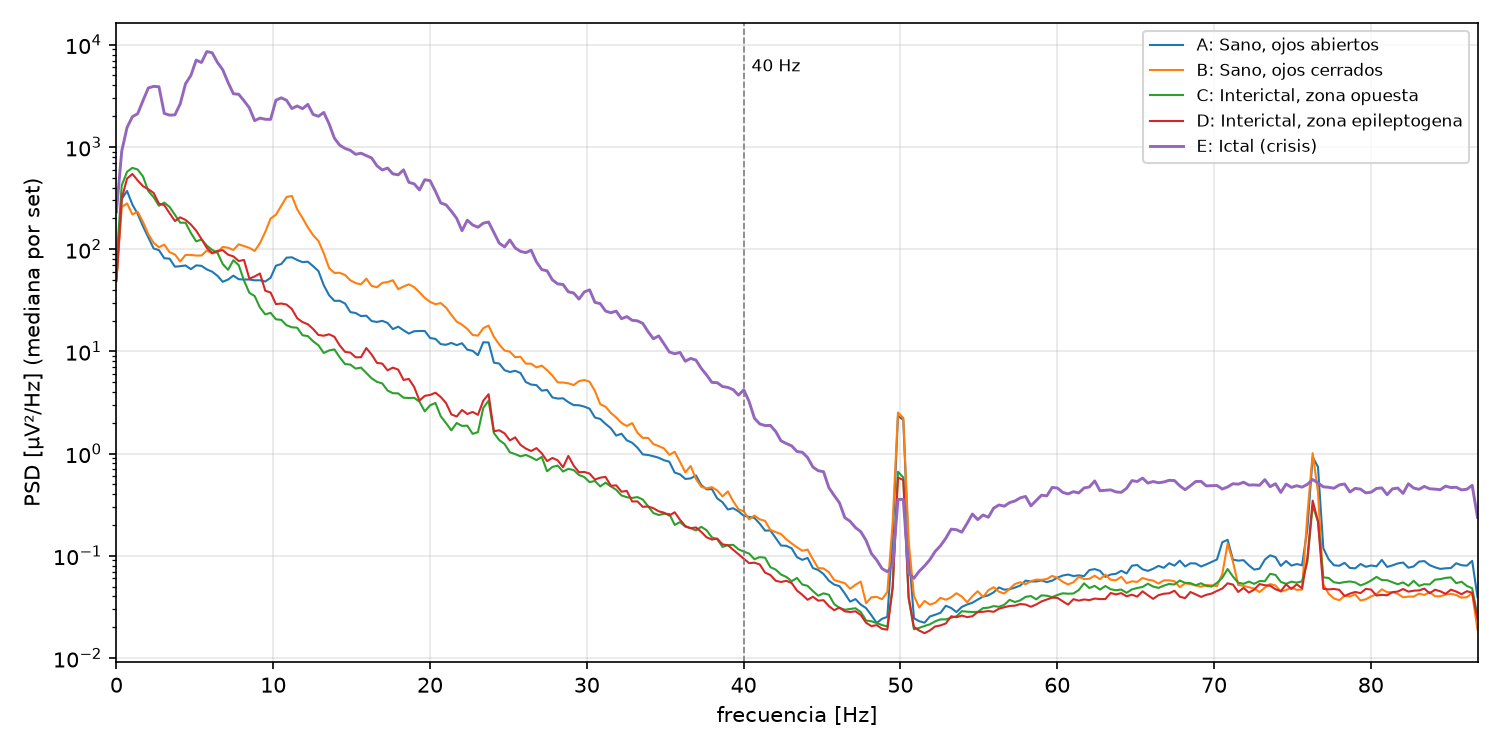
\includegraphics[width=0.85\textwidth]{etapa1/psd_welch_por_set.png}
  \caption{Densidad espectral de potencia (Welch, Hann de 512 muestras, 50~\% de solapamiento), mediana por
           set de Bonn, antes del filtro de 40 Hz.}
  \label{fig:psd_bonn}
\end{figure}

\begin{table}[ht]
\centering
\caption{Potencia relativa media por banda en cada set de Bonn (señal filtrada a 40 Hz). Cada fila suma 1.}
\label{tab:bonn_bandas}
\begin{tabular}{llrrrrr}
\toprule
Set & Descripción & delta & theta & alfa & beta & gamma \\
\midrule
A & sano, ojos abiertos     & 0,367 & 0,182 & 0,241 & 0,203 & 0,007 \\
B & sano, ojos cerrados     & 0,181 & 0,126 & \textbf{0,476} & 0,213 & 0,004 \\
C & interictal, zona opuesta & \textbf{0,668} & 0,214 & 0,071 & 0,044 & 0,002 \\
D & interictal, foco        & 0,602 & 0,253 & 0,100 & 0,044 & 0,001 \\
E & ictal                   & 0,248 & \textbf{0,405} & 0,174 & 0,171 & 0,003 \\
\bottomrule
\end{tabular}
\end{table}

La Tabla~\ref{tab:bonn_bandas} muestra que la \emph{distribución} de la potencia entre bandas también
cambia: en el set E la banda dominante es theta (40,5~\%), mientras que en los interictales intracraneales
(C, D) domina delta (60--67~\%). El espectrograma de un segmento ictal (Figura~\ref{fig:espectrograma_bonn})
muestra además que la frecuencia de la descarga no es constante a lo largo del tiempo.

\begin{figure}[ht]
  \centering
  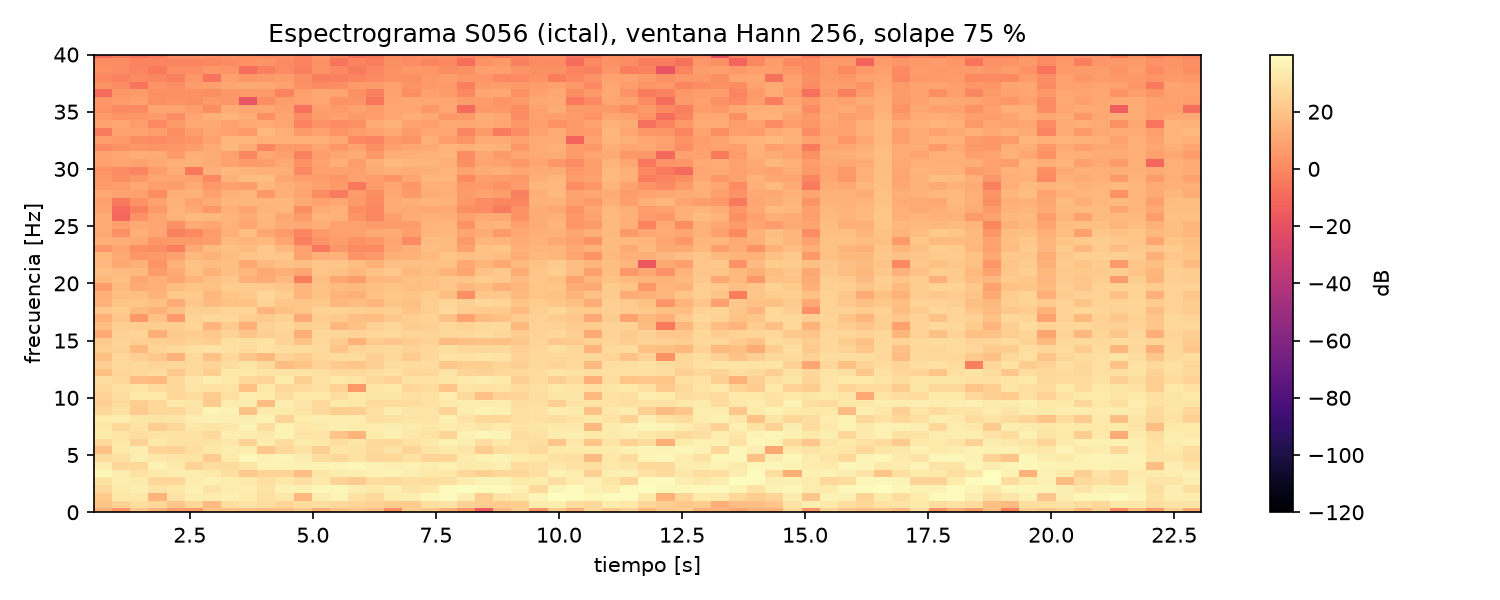
\includegraphics[width=0.85\textwidth]{etapa1/espectrograma_S056.png}
  \caption{Espectrograma del segmento ictal S056 de Bonn (Hann de 256 muestras, 75~\% de solapamiento).}
  \label{fig:espectrograma_bonn}
\end{figure}
